\documentclass[9pt]{beamer}
\usepackage{latex-course}

% Define Layout
\usetheme[compress]{Berlin}
\useinnertheme{circles}
\useoutertheme{miniframes}

\beamertemplatenavigationsymbolsempty
\setbeamertemplate{blocks}[rounded][shadow=true]













\AtBeginSection[]
{
	\begin{frame}{}
	   {\Huge \insertsectionhead}
		\begin{multicols}{2}	
		\tableofcontents[currentsection,hideothersubsections]
	\end{multicols}
   \end{frame}
}




% Define a block for the code examples
\newenvironment<>{codeblock}[1]{%
  \begin{actionenv}%
      \def\insertblocktitle{#1}%
      \par%
      \mode<presentation>{%
        \setbeamercolor{block title}{fg=white,bg=orange!20!black}
       \setbeamercolor{block body}{fg=black,bg=olive!50}
       \setbeamercolor{itemize item}{fg=orange!20!black}
       \setbeamertemplate{itemize item}[triangle]
     }%
      \usebeamertemplate{block begin}
 }{
 	\par\usebeamertemplate{block end}\end{actionenv}
}




%% Display a code example
% Usage: \codex[(no-)preview]{title}{file-basename}
\newcommand{\codex}[3][include]{
	% Create the header
	\label{codex:#3}
	\begin{codeblock}{#2 \hfill \tiny{(\href{run:../code/#3.tex}{Code}
				\ifthenelse{\equal{#1}{no-preview}}{}{,
		\href{run:../code/#3.pdf}{PDF}})}}
	
	% Start the columns when a preview is wanted
	\ifthenelse{ \equal{#1}{no-preview} }{}{
		\begin{columns}[onlytextwidth]
		\column{0.49\linewidth} }

	% Main Job: Include the code!
	\lstinputlisting{#3.tex}

	% Only include preview and columns of wanted
	\ifthenelse{ \equal{#1}{no-preview} }{}{
		\column{0.49\linewidth}
			\ifthenelse{ \equal{#1}{no-preview} }{ 
				% only include if preview is wanted
			}{
				\mimage{#3-crop.pdf}
			}
		\end{columns}
	}
	\end{codeblock}
}

%% Display bibtex codeblock
\newcommand{\codexBibtex}[2]{
	\begin{codeblock}{#1 \hfill \tiny{(\href{run:../code/#2.bib}{Code})}}
		\lstinputlisting{#2.bib}
	\end{codeblock}
}

\newcommand{\inote}[1]{\note[item]{#1}}


\makeatletter
\author[manuel@gobics.de]{\@author}
\institute[http://www.gobics.de]{Manuel Landesfeind\\Department of Bioinformatics\\Institute for Microbiology and Genetics\\University of G\"ottingen}
\date[07.-10.04.2015]{April 7th to 10th 2015}
\makeatother


\begin{document}
\maketitle
\section{Introduction}
\subsection{About \LaTeX}

\begin{frame}
	\begin{columns}[onlytextwidth]
		\column{0.59\linewidth}
			\mquote{Wikipedia}{\LaTeX{} is a document markup language and document preparation system for
			the \TeX{} typesetting program.}
			\begin{itemize}
				 \item 1987 - Donald E. Knuth developed \TeX{} (Setter) for writing his book
				''The art of computer programming''
				\item  1994 - \LaTeX{} (Layout) is developed by Leslie Lamport for
					easier use of {\TeX}
				\item  Active community develops \LaTeX{} makros and additional packages.
			\end{itemize}
		\column{0.39\linewidth}
			\mimage{latex_stack.pdf}
	\end{columns}
\end{frame}

\subsection{Why developing texts in \LaTeX{}}
\begin{frame}
	\begin{block}{Devide writing and layout}
		While writing \LaTeX{} the final layout is not visible immediately
		(opposed to WYSIWYG word processors). 
		\begin{itemize}
			\item focuses the writer on the writing, thus more productive
				\inote{writer is not distracted by the layout}
			\item special typesetting (e.g. sigils)
				\inote{many letter \todo{Folgen} are better readable if the 
					were rendered special e.g. ff}
		\end{itemize}
	\end{block}

	\begin{block}{Portability}
		Simple text-files can be opened with any editor in any operating 
		system.
		\inote{ever tried to open a docX file from work on your home PC with
		an older MS Office version?}
		\inote{text files can also be opened in 10 years}
	\end{block}
\end{frame}

\subsection{Resources}
\begin{frame}

	\begin{itemize}
		\item CTAN \url{http://www.ctan.org/}\\
			the \emph{C}omprehensive \emph{T}eX \emph{A}rchive \emph{N}etwork
		\item LaTeX Wikibook\\
			\url{http://en.wikibooks.org/wiki/LaTeX}

		\item \LaTeX{} templates\\
			\url{http://www.latextemplates.com}
	\end{itemize}
\end{frame}


\subsection{Writing a \LaTeX{} document}
\begin{frame}
\begin{center}
	\mimage[width=0.6\textwidth]{latex_compile_process.pdf}
\end{center}
\end{frame}


\subsection{Available Software}
\begin{frame}
	\frametitle{\LaTeX packages}

	\begin{block}{Texlive (Linux)}
		Available in all distributions, e.g. Ubuntu, Suse Linux. Install it
		from your software center (attention: several packages may be
		required).
	\end{block}
	\begin{block}{MiKTeX (Windows)}
		Freely available at \url{http://www.miktex.org}.
	\end{block}	
	\begin{block}{MacTeX (Mac OS)}
		Freely available at \url{http://www.tug.org/mactex}.
	\end{block}
\end{frame}

\subsection{\LaTeX{} editors}
\begin{frame}

	\inote{Remember: What is the difference between a text-editor and -processor?}
	Every simple text-editor can be used but more comfortable:

	\begin{columns}[T,onlytextwidth]
	\column{0.49\textwidth}
		\begin{block}{TeXMaker}
			\url{http://www.xm1math.net/texmaker}
			\begin{itemize}
				\item free and cross-platform editor
				\item syntax highlightning
				\item compile via mouse click
				\item displays previews
			\end{itemize}
		\end{block}
	\column{0.49\textwidth}
		\begin{block}{Kile}
			\url{http://kile.sourceforge.net}
			\begin{itemize}
				\item integrated {\LaTeX} environment
				\item easily installed on all Linux distributions
			\end{itemize}
		\end{block}
	\end{columns}

	\vfill

	\begin{block}{Mobile devices}
		Editors for mobile devices can be found in the Play/App Store
		(may require web-access to compile the documents).
	\end{block}
\end{frame}
\subsection{Creation using the Texmaker IDE}
\begin{frame}
	\begin{enumerate}
		\item Start Texmaker
		\item create a new document
		\item insert basic information
		\item compile and view
	\end{enumerate}

	\mimage{texmaker-intro.pdf}
\end{frame}

\subsection{A first example}
\begin{frame}
	\codex{Basic document}{basic-document-np}
	\begin{itemize}
		\item \lcs{documentclass} defines the type of the text e.g. book,
			article, report
		\item \len{document} contains the actual text (the part
			before is called \emph{preamble})
		\item \lcs{maketitle} produces a basic heading
	\end{itemize}
\end{frame}
\subsection{Names and ...}
\begin{frame}
	\begin{description}
		\item[package] is an additional \LaTeX{} plugin with a special purpose
			(e.g. for images, specific mathematical/chemical formulas)
		\item[command] specific modification of the document by the means of
			the given command, e.g. emphasizing a text or bold/italic font.
		\item[environment] specific modification of a longer part of the text,
			e.g. centering a paragraph.
	\end{description}
\end{frame}



\subsection{Compiling documents}
\begin{frame}
	Resulting file formats are
	\href{http://en.wikipedia.org/wiki/Page_description_language}{\emph{page description
	format}} files:
	\begin{block}{File formats}
		\begin{description}
			\item[DVI] Device independent file format\\
				\url{http://de.wikipedia.org/wiki/Device_independent_file_format}
			\item[PS] PostScript\\
				\url{http://de.wikipedia.org/wiki/PostScript}
			\item[PDF] Portable Document Format\\
				\url{http://en.wikipedia.org/wiki/PDF}
		\end{description}
	\end{block}

	\begin{block}{Using PDFLaTeX on the command line}
		\code{pdflatex document.tex}
		It is preferable to execute the command twice because specific parts
		of the document are first correct after the second run.
	\end{block}
\end{frame}

\section{Basic typography}

\subsection{Getting started with {\LaTeX}}
\begin{frame}
	\begin{block}{Document class}
		\lcs{documentclass} specifies the type of the document and basic
		layout options. Available document classes are:
		\begin{description}
			\item[article] for journal articles and small texts
			\item[report] longer text e.g. thesis, small books
			\item[book] with parts and chapters
			\item[letter] for old-school communication
			\item[beamer] for presentations (see later)
		\end{description}
	\end{block}

	\begin{block}{German Layouts}
		For a more feasible german layout the KOMA-Script classes can be
		used\footnote{\url{http://www.ctan.org/pkg/koma-script}}:
		\begin{center}\begin{tabular}{l@{$\rightarrow$}r}
		article & scrartcl\\
		 report & scrreprt\\
		book & scrbook
		\end{tabular}\end{center}
	\end{block}
\end{frame}
\begin{frame}
	\begin{block}{Commands}
		Can be used to modify the text, include images and everything else.
		A command
		\code{{\textbackslash}command[optional argument(s)]\{required
		argument\}}
		always start with a backslash ''\textbackslash'' followed by the
		command name. Optional and/or required arguments may be added.
	\end{block}
	An already known command is the \lcs{documentclass} but now with more
	details:
	\code{\textbackslash{}documentclass[9pt,a4paper,twosided,draft]\{article\}}
\end{frame}
\begin{frame}
	\begin{block}{{\LaTeX} groups}
		Some (low-level) arguments do not take arguments but effect more than
		you would expect
		\codex{Without grouping}{commands-without-restriction}
		This can be changed by using braces to build groups
		\codex{Now with grouping}{commands-without-restriction-2}
	\end{block}
	\inote{Emphasize on the missing space after {\LaTeX}, the expanded TT-Font
	and the full centering of all the text.}
\end{frame}
\begin{frame}
	\begin{block}{{\LaTeX} environments}
		Used to modify blocks of content (e.g. centering text):
		\codex{Aligning text}{text-align}
	\end{block}
\end{frame}
\begin{frame}
	\begin{block}{{\LaTeX} packages}
		Additional plugins/modules called \emph{packages} can be included for
		more features like
		\begin{multicols}{2}
			\begin{itemize}
				\item inlcuding images
				\item extra-long tables
				\item mathematical formulas
				\item drawing chemical structure formulas
				\item spliting list in multiple rows (as demonstrated here)
			\end{itemize}
		\end{multicols}
	\end{block}

	\begin{block}{Using packages}
		Packages need to be included with
		\code{{\textbackslash}usepackage[optional arguments]\{package name\}}
		e.g. for easy including images:
		\code{{\textbackslash}usepackage\{graphicx\}}
	\end{block}

	A full list of available packages is available at
	\url{http://www.ctan.org/pkg}
\end{frame}

\subsection{More {\LaTeX} characteristics}
\begin{frame}
	\begin{block}{Whitespaces}
		Multiple whitespaces (e.g. space, tab-space, enter) are ignored in
		\LaTeX{}
	\end{block}
	\codex{Newlines can be added manually}{newlines}
\end{frame}

\begin{frame}
	\begin{block}{Comments}
		Additional text, that is not displayed at the end can be added
		after \%
	\end{block}
	\codex{Comment example}{comment}
\end{frame}

\begin{frame}
	\begin{block}{Special characters}
		{\LaTeX} uses special characters e.g. ''\textbackslash'' to start
		commands or ''\%''
		for comments. If these symbols should be printed, they need to be 
		escaped.
	\end{block}
	\codex{Special characters require escaping}{special-characters}

	\LaTeX{} provides support for $> 5000$ symbols which are listed at 
	\url{http://www.ctan.org/pkg/comprehensive}
\end{frame}

\subsection{Structuring text}
\begin{frame}
	\codex{Structures}{structures}
\end{frame}
\begin{frame}
	\codex{Table of contents}{tableofcontents}
	Further available commands are \lcs{listoffigures} and \lcs{listoftables}.
\end{frame}

\subsection{Lists}
\begin{frame}
	\codex{Enumeration}{enumerate}
\end{frame}
\begin{frame}
	\codex{Item list}{itemize}
\end{frame}
\begin{frame}
	\codex{Description}{description}
\end{frame}

\subsection{Font formatting}
\begin{frame}
	\begin{alertblock}{Warning}
		It is strongly discouraged to perform direct formatting of text! Later
		we will learn better methods. Nevertheless, these commands are needed
		and therefore listed here.
	\end{alertblock}

	The creation of new commands to wrap semantics into layouts is described
	later.
\end{frame}
\begin{frame}
	\codex{Different font sizes}{font-size}
\end{frame}

\begin{frame}
	\codex{Direct format of text}{font-format}
\end{frame}

\begin{frame}
	Fonts have to be prepared for {\LaTeX} therefor it can not use the normal
	fonts on the system.

	\begin{block}{Font types}
		{\LaTeX} provides a variety of fonts as listed on
		\url{http://www.tug.dk/FontCatalogue}
	\end{block}

	\begin{block}{True-Type fonts}
		System fonts (mostly TTF) can be incorporated in {\LaTeX} which is not
		explained here. Please refer to
		\href{http://en.wikibooks.org/wiki/LaTeX/Fonts}{the {\LaTeX} WikiBook}
	\end{block}
\end{frame}

\section{Tables}

\subsection{Defining a basic table}
\begin{frame}
	\begin{block}{Basic table creation}
		Tables are build with the \len{tabular} environment. This needs a
		parameter defining the number of columns and their alignment:
		\code{\textbackslash{}begin\{tabular\}\{column identifier\}}
	\end{block}

	Generally, creating tables in {\LaTeX} is not straightforward. Tools to
	create tables will be explained later.
\end{frame}

\begin{frame}
	\plabel{frm:tabular-column-identifier}
	\begin{block}{Column identifier}
		Is a text containing of alignment or line information:
		\begin{mitemize}
			\item l --- a normal column
			\item c --- a centered column
			\item r --- a right aligned column
			\item \textbar --- a vertical border
		\end{mitemize}
	\end{block}
	\begin{exampleblock}{Some examples on columns}
		\begin{itemize}
			\item \color{code}{l\textbar{}ccc}\\
				4 columns. In every row, the first cell is left aligned and the other are
				centered. A vertical border is drawn between the first and
				second cell.
			\item \color{code}{\textbar{}lccr\textbar{}}
				Every row contains 4 cells, where the first is left and the
				fourth is right aligned. The two cells in the middle are
				centered. There a vertical borders before and after the row.
		\end{itemize}
	\end{exampleblock}
\end{frame}

\begin{frame}
	\begin{block}{Table contents}
		Full {\LaTeX} support with special syntax for
		\begin{mdescription}
			\item[\&] creates a new cell
			\item[\textbackslash\textbackslash{}] new row
			\item[\lcs{hline}] create a horizontal line
			\item[\lcs{newline}] a new line within the \emph{current cell}
		\end{mdescription}
	\end{block}

	\codex{Basic table}{tabular-basic}
\end{frame}

\subsection{Paragraph columns}
\begin{frame}
	
	Columns with a very long text (e.g. description) may be longer
	than the available page space.
	
	\codex{Column with overfill}{tabular-column-p-1}

\end{frame}
\begin{frame}
	\begin{block}{Paragraph columns}
		Paragraph columns perform automatic line breaking and have a defined
		with:
		\begin{mdescription}
			\item[p\{width\}] text aligned to top of cell
			\item[m\{width\}] text in the middle
			\item[b\{width\}] text to bottom
		\end{mdescription}
	\end{block}
	\codex{Column with overfill (revised)}{tabular-column-p-2}
\end{frame}
\begin{frame}
	\begin{block}{The \lp{tabularx} package}
		This package introduces the \len{tabularx} and \emph{X} column identifier with automatic
		calculation for the required size.
	\end{block}
	\codex{Usage of the \lp{tabularx} package}{tabular-tabularx}
\end{frame}

\subsection{Borders and lines}
\begin{frame}
	\begin{block}{More horizontal lines}
		The \lcs{cline\{i-j\}} command creates a border from the cell $i$ to $j$
	\end{block}
	\codex{Example using \lcs{cline}}{tabular-cline}
\end{frame}
\begin{frame}
	\codex{Using @ to define the cell separator}{tabular-column-at}
\end{frame}

\subsection{Spanning rows, columns, and tables}
\begin{frame}
	\codex{Spanning multiple columns}{tabular-multicolumn}
	\lcs{multicolumn} requires three arguments
	\begin{menumerate}
		\item number of columns to span
		\item text alignment (see slide \pageref{frm:tabular-column-identifier})
		\item content of the spanned cell
	\end{menumerate}
\end{frame}
\begin{frame}
	\codex{Spanning multiple row}{tabular-multirow}
	\code{\textbackslash{}multirow\{num rows\}\{width\}\{content\}}
\end{frame}
\begin{frame}
	\codex{Spanning a table to multiple pages}{tabular-longtable}
\end{frame}

\subsection{Tools to generate {\LaTeX} tables}
\begin{frame}
	\begin{block}{Calc2Latex}
		Macro for Libre-/OpenOffice:
		\url{http://sourceforge.net/projects/calc2latex}
		After installation, select parts to export and run the \emph{Main}
		macro.
	\end{block}

	\begin{block}{Excel2LaTeX\hfill{\small (untested)}}
		Add-In for Excel is available at:
		\url{http://www.ctan.org/tex-archive/support/excel2latex}
	\end{block}

	\begin{block}{Webservice converter}
		An online converter is available at:
		\url{http://www.tablesgenerator.com/}
	\end{block}
\end{frame}

\subsection{Useful hints}
\begin{frame}
	\begin{block}{Long words}
		{\LaTeX} never hyphenates the first word of a paragraph. To disable this in tables use \lcs{hspace\{0cm\}}.
	\end{block}
	\begin{block}
		Generated tables sometimes use a lot of unnecessary \lcs{multirow} commands. Check the generated tables.
	\end{block}
\end{frame}

\begin{frame}
	\begin{block}{Commands for every cell}
		It is possible to include a command before and after the content of every cell using the \lsc{>\{\textbackslash{}cmd\}} and \lsc{<\{\textbackslash{}cmd\}} syntax of the lp{array} package. This can be combined with \lcs{newcolumntype\{\}\{\}}.
	\end{block}
	\codex{centered tabularx}{tabular-tabularx-centered}
\end{frame}
\section{Images and graphics}

\subsection{Excursion on image types}
%\begin{frame}
%	\begin{block}{Color spectra in informatics}
%		
%	\end{block}
%\end{frame}

\begin{frame}
	\begin{columns}[onlytextwidth]
	\column{0.6\textwidth}
		\begin{block}{Bitmap-Images}
			Every image/graphic consists of a specific $length$ and $width$. It is
			separated into a grid of \emph{dots} (or \emph{pixel}):
			Classically, for every dot the corresponding color is stored:
		\end{block}
			
		\begin{exampleblock}{Examples}
			\begin{itemize}
				\item \href{http://de.wikipedia.org/wiki/JPEG}{Joint
					Photographic Experts Group format (JPEG)}
				\item \href{http://de.wikipedia.org/wiki/Portable_Network_Graphics}{Portable Network
					Graphics (PNG)}
				\item \href{http://de.wikipedia.org/wiki/GIF}{Graphics
					Interchange format (GIF)}
			\end{itemize}
		\end{exampleblock}
	\column{0.38\textwidth}
		{\centering\mimage{graphics-dots-explained.pdf}}

		{\tiny derived from \href{http://commons.wikimedia.org/wiki/File:Aufloesung\_erklaert.svg}{CC-BY-SA
		v3.0 by Friedrich Graf}}
	\end{columns}
\end{frame}

\begin{frame}
	\begin{columns}[onlytextwidth]
	\column{0.38\textwidth}
		\mimage{graphics-svg-explained.pdf}
	\column{0.6\textwidth}
		\begin{block}{Vector graphics}
			Store information about elements (e.g. circles and lines) to be drawn, with information
			about the size and relation to each other.
		\end{block}
		\begin{exampleblock}{Examples}
			\begin{itemize}
			\item \href{http://de.wikipedia.org/wiki/SVG}{Scalable Vector Graphics (SVG)}
			\item \href{http://de.wikipedia.org/wiki/Portable_Document_Format}{Portable	Document Format (PDF)}
			\end{itemize}
		\end{exampleblock}
	\end{columns}
\end{frame}

\begin{frame}
	\begin{block}{Comparing bitmap and vector graphics}
		Vector graphics can be scaled to whatever size without loss of
		precision.
	\end{block}

	\begin{columns}[onlytextwidth]
	\column{0.49\textwidth}
		\begin{exampleblock}{PNG image at 5, 50, 100 pixel size}
			
\includegraphics[width=5px]{default-image.png}
			
\includegraphics[width=50px]{default-image.png}
			
\includegraphics[width=100px]{default-image.png}
		\end{exampleblock}
	\column{0.49\textwidth}
		\begin{exampleblock}{PDF image at same sizes}
			
\includegraphics[width=5px]{default-image.pdf}
			
\includegraphics[width=50px]{default-image.pdf}
			
\includegraphics[width=100px]{default-image.pdf}
		\end{exampleblock}
	\end{columns}
\end{frame}
		
\subsection{Including graphical images}
\begin{frame}
	\begin{block}{Using the \lp{graphicx} package}
		Images can be included with the \lcs{includegraphics} command.
		They can be stored at different locations provided by \lcs{graphicspath}.
	\end{block}
	\codex{Simple image inclusion}{includegraphics}
	{\tiny \href{../doc/graphicx.pdf}{(Graphixs-Documentation)}}
\end{frame}
\begin{frame}
	\codex{Including scaled images}{includegraphics-scaled}
\end{frame}
\begin{frame}
	\codex{Including images with defined with and height}{includegraphics-textwidth}
\end{frame}
\begin{frame}
	\codex{Display part of image}{includegraphics-viewport}
\end{frame}

\section{Floating environments}
\subsection{On floats}
\begin{frame}
	Floats are containers for images, tables, and user-defined contents
	\begin{columns}[c]
	\column{0.4\textwidth}
	\begin{itemize}
		\item auto-placed: floats do not appear at the position they are
			defined
		\item un-broken: a float can/will not stretch over more than 1
			page
	\end{itemize}
	\column{0.59\textwidth}
	Available by default: 
	\begin{itemize}
		\item \len{figure}
		\item \len{table}
	\end{itemize}
	\end{columns}
\end{frame}

\begin{frame}
	\begin{block}{Caption}
		\lcs{caption} adds a caption to the current float, via
		\code{\textbackslash{}caption[short variant]\{My caption\}}
	\end{block}

	\begin{block}{Float counter}
		Every float environment has an own counter for later reference.
	\end{block}
\end{frame}

\subsection{The figures float}
\begin{frame}
	Used for graphics...
	\codex{Graphic in a figure float}{figure}
\end{frame}


\subsection{The table float}
\begin{frame}
	... And for tables.
	\codex{A table in a float}{table}
\end{frame}

\subsection{Placing the floats}
\begin{frame}
	\codex{Defining a specific placement}{floats-placement}

	\begin{description}
		\item[h] places the float approximately here
		\item[t] at the top of a page
		\item[b] at the bottom of a page
		\item[p] put floats together on a page containing only floats
		\item[H] put the float exactly here (requires \lp{float} package)
	\end{description}
\end{frame}
\subsection{More layout options with floats}
\begin{frame}
	\codex{Captions on the side}{floats-sidecap}
\end{frame}
\begin{frame}
	\codex{Wrapping text around figures}{floats-wrapfig}
\end{frame}
\begin{frame}
	\codex{Having subfloats}{floats-subfloats}
\end{frame}

\subsection{Creating an index for floats}
\begin{frame}
	Creating an index of figures and tables is trivial:
	\codex{Index of the figures used}{listoffigures}
	Lists of tables are created with the \lcs{listoftables}
\end{frame}
\begin{frame}
	Also own floats can be printed as list
	\codex{List of own floats}{float-listof}
\end{frame}
\begin{frame}[plain]
	\warn{List generally are not displayed in the the table of contents!}
	\codex{Including list into the table of
	contents}{tableofcontents-include-other-lists}
	The \lcs{phantomsection} is required for the correct page number.
	\lcs{addcontentsline} creates label to be references.
\end{frame}


\subsection{Creating new floats}
\begin{frame}
	\codex{Creating a custom float for computer source code}{floats-custom-np}
\end{frame}
\begin{frame}
	\begin{itemize}
		\item \lcs{floatstyle} - define the default style for new floats\\
			\begin{itemize}
				\item plain - normal layout
				\item plaintop - normal layout with caption above float
				\item boxed - a box around the float with caption outside
				\item ruled - using rules (see example)
			\end{itemize}
		\item \lcs{newfloat} - creates the new float with the given name\\
			\code{\textbackslash{}newfloat\{name\}\{placement
					identifiers\}\{listname\}[outer
				counter name]}
				Captions are written to the \texttt{listname} file to be used in
				lists. If outer counter is given it will prefix the counter
				(e.g. chapter, section)
		\item \lcs{floatname} - set name for new float
	\end{itemize}
\end{frame}

\subsection{Layout captions}
\begin{frame}
	Extended format specifications via the
\href{http://www.ctan.org/pkg/caption}{\lp{caption}}

	\codex{Decrease caption indent}{captionsetup}
\end{frame}


\section{Mathematical formulas}
\subsection{Introduction}
\begin{frame}
	\LaTeX{} has been developed to typeset especially mathematical text
	documents containing also (very complex) formulas, e.g.
	$$ \mathbf{B} = \frac{\mu_0}{4\pi}\int_C \frac{I d\mathbf{l} \times \mathbf{\hat r}}{|\mathbf{r}|^2} $$
	or
	$$ \mathbf{E} = \frac{q}{4\pi \epsilon_0} \frac{1-\frac{v^2}{c^2}}{(1-v^2\sin^2\theta/c^2)^{3/2}}\frac{\mathbf{\hat	r}}{r^2}$$
\end{frame}

\subsection{The math-environment}
\begin{frame}
	\LaTeX{} distinguishes between normal text and math mode.

	\codex{Using \$ and \$\$}{mathmode}
\end{frame}
\begin{frame}
	\codex{Using eqnarray}{eqnarray}
\end{frame}
\begin{frame}
	\codex{Using eqnarray with labels}{eqnarray-label}
\end{frame}

\subsection{Basic math}
\begin{frame}
	\begin{block}{Usefull packages}
		\lp{amsmath},\lp{amsfonts},\lp{amssymb}, \lp{amstext}
	by the American Mathematical Society\footnote{\url{http://www.ams.org}}
	\end{block}
\end{frame}
\begin{frame}
	\LaTeX{} supports mostly normal math:
	\codex{Basic operations in math}{math-basic}
\end{frame}
\begin{frame}
	\codex{Comparing digits}{math-compare}
\end{frame}
\begin{frame}
	\codex{Complex formulas with symbols}{math-symbols}
\end{frame}

\subsection{Parentheses}
\begin{frame}
	\codex{Parentheses with \lcs{left} and \lcs{right}}{parentheses}
	\codex{One-sided parentheses}{parentheses-right-dot}
\end{frame}


\subsection{Text in the math mode}
\begin{frame}
	\codex{Display normal text in math}{math-text}
\end{frame}

\subsection{More on {\LaTeX} math mode}
\begin{frame}
	A very intense overview over symbols etc. at
	\begin{center}
		\url{http://en.wikipedia.org/wiki/Help:Displaying_a_formula}
	\end{center}
	Drawn symbols can be recognized and possible \LaTeX commands proposed at
	\begin{center}
		\url{http://detexify.kirelabs.org/classify.html}
	\end{center}
\end{frame}

\section{References}
%openout_any = r has to be set in texmf.cnf somewhere deep in the config files for the Makefile to work with references.

\subsection{Basic labels and references}
\begin{frame}
	\begin{block}{Labels}
		Labels are used to reference the last statement, e.g. a section:
	\end{block}
	\codex{Label for a section}{label-section}

	\begin{block}{Labels revised}
		Because labels are just strings it is a ''best practice'' to use a prefix, e.g.
	\end{block}
	\codex{Section label with prefix}{label-section-prefix}
\end{frame}

\begin{frame}
	\begin{block}{Referencing labels}
		To reference a label use the \lcs{ref} command:
	\end{block}
	\codex{Simple referencing using \lcs{ref}}{label-ref}
\end{frame}

\begin{frame}
	Often a reference to a specific paragraph is required

	\codex{Referencing a \lcs{phantomsection}}{label-phantomsection}

\end{frame}

\subsection{Easier referencing with prefixes}
\begin{frame}
	The prefixes are used to determine the type of the reference and a custom
	description is added
	\codex{Using the \lp{prettyref} package}{prettyref}

	To define a new prefix, the command 
	\code{\textbackslash{}newrefformat\{prefix\}\{format\}}
	is used.
\end{frame}

\subsection{References to figures and tables}
\begin{frame}
	\begin{block}{Referencing figures}
		Also images and tables can be references. \emph{Warning:} 
		\lcs{label} always \emph{after} the \lcs{caption} command
	\end{block}
	\codex{Referencing an image (correct and wrong)}{label-image}
\end{frame}
\begin{frame}
	Also figures and tables can be referenced with \lp{prettyref}:
	\codex{Referencing a figure with \lcs{prettyref}}{prettyref-figure}
\end{frame}

\subsection{Clickable links}
\begin{frame}
	\begin{block}{Clickable links}
		With support of the \lp{hyperref} package the PDF output will contain
		clickable links.
	\end{block}
	\codex{Using the \lcs{nameref} command}{nameref}
\end{frame}
\begin{frame}
	\codex{Linking a website}{url}
	\codex{Linking an email}{url-mailto}
\end{frame}
\begin{frame}
	With \lp{hyperref}, \lcs{url}, and \lcs{href} also PDFs and files can be linked:
	\codex{Linking a PDF and video with \lcs{href}}{url-file}
\end{frame}

\section{Bibliography with Bib\TeX{}}

\subsection{{\LaTeX} build in bibliography}
\begin{frame}
	Built in support for references using the \len{thebibliography} and
	\lcs{cite} command
	\codex{References using the build in bibliography}{thebibliography}
\end{frame}
\begin{frame}
	\codex{References using the build in bibliography (define cite name)}{thebibliography-names}
\end{frame}

\subsection{Using a Bib{\TeX} library}
\begin{frame}
	The more {\LaTeX} way is a separate library using {Bib\TeX}
	\codexBibtex{{Bib\TeX} library file}{bibtex-library}
	Commands are located where the final bibliography will be included.
\end{frame}
\begin{frame}
	\codex{Using the library in {\LaTeX}}{bibtex-bibliography}
\end{frame}
\begin{frame}
	Compiling {\LaTeX} with {Bib\TeX} requires extra effort
	\begin{columns}[onlytextwidth]
		\column{0.35\textwidth}
		\lstinputlisting[language=bash,keywords={pdflatex,bibtex}]{compile-with-bibtex.sh}
		\column{0.64\textwidth}
			\begin{enumerate}
				\item create basic output file\\
					\texttt{\tiny LaTeX Warning: Citation `lamport94' on ...
					undefined}
				\item include bibliography
				\item compile with the bibliography\\
					\texttt{\tiny LaTeX Warning: Label(s) may have changed. Rerun
					...}
				\item ensure the cross-references to be right
			\end{enumerate}
	\end{columns}
\end{frame}


\subsection{Using the \textbackslash{}cite command}
\begin{frame}
	\codex{Citing with optional argument}{cite-optional}
\end{frame}
\begin{frame}
	Default {\LaTeX} bibliography uses numerical references (often used in
	mathematics/computer science).

	\codex{\lp{natbib} package supports named citing}{cite-natbib}

	More possible commands are: \lcs{citep}, \lcs{citet*}, \lcs{citep*}

	\warn{Natbib does not work with numerically referenced bibliographies}
\end{frame}


\subsection{Selecting an appropriate {Bib\TeX} style}
\begin{frame}
	Different styles can be used to produce different views
	\begin{center}
		\begin{tabular}{l|l|l|l}
		\multicolumn{1}{c|}{Style Name} & \multicolumn{1}{c|}{Author Name Format} & \multicolumn{1}{c|}{Reference Format} & \multicolumn{1}{c}{Sorting} \\ \hline
		plain & Homer Jay Simpson & \#ID\# & by author \\ \hline
		unsrt & Homer Jay Simpson & \#ID\# & as referenced \\ \hline
		abbrv & H. J. Simpson & \#ID\# & by author \\ \hline
		alpha & Homer Jay Simpson & Sim95 & by author \\ \hline
		abstract & Homer Jay Simpson & Simpson-1995a &  \\ \hline
		acn & Simpson, H. J. & \#ID\# &  \\ \hline
		authordate1 & Simpson, Homer Jay & Simpson, 1995 &  \\ \hline
		apa & Simpson, H. J. (1995) & Simpson1995 &  \\ \hline
		named & Homer Jay Simpson & Simpson 1995 &  \\ \hline
		\end{tabular}
	\end{center}

	More styles at
	\url{http://www.cs.stir.ac.uk/~kjt/software/latex/showbst.html}

\end{frame}

\subsection{Creating your own style for {Bib\TeX}}
\begin{frame}
	\begin{block}{Bib{\TeX} style files}
		{Bib\TeX} libraries do not contain style information (only structured
		information). 

		Styles are stored as {\color{code}.bst} files (pure text).
	\end{block}

	\begin{block}{Creating an own style}
		Simply execute \code{latex makebst} on the command line and respond to
		the questions asked.

		\textbf{Note:} Answering the last question ''Shall I now run this batch
		job?'' with yes or executing it by yourself:
		\code{latex my-style.dbj}
		will result in a {\color{red}my-style.bst} (the actual style file).
	\end{block}

\end{frame}

\subsection{Editing bibliography graphically}
\begin{frame}
	JabRef may be used to edit a {Bib\TeX} library
	\begin{center}
		\mimage{ss-jabref.png}

		\url{http://jabref.sourceforge.net}
	\end{center}	
\end{frame}


\begin{frame}
	Also \href{http://www.zotero.org}{Zotero} can export {Bib\TeX}
	\begin{center}
		\mimage{ss-zotero-export.png}
	\end{center}
\end{frame}

\subsection{Bib{\TeX} is supported by many online platforms}
\begin{frame}
	As {\LaTeX} is used extensively in academia, many online sources support Bib{\TeX}.
	
	JabRef can import several outside sources and Google Scholar provides Bib{\TeX} code:
		\begin{center}
		\mimage{bibtex_google_scholar.pdf}
	\end{center}
\end{frame}

\section{Customizing {\LaTeX}}

\subsection{Writing own commands}
\begin{frame}
	New commands can be created with the \lcs{newcommand} or redefined with
	the \lcs{renewcommand}.
	\codex{Creating a command for simpler quotes}{newcommand-quotes}
	\code{\lcs{newcommand}\{\textbackslash{}name\}[num params]\{definition\}}
	\pause
	\codex{Creating a command to display organism names}{newcommand-ecoli}
\end{frame}
\begin{frame}
	\codex{Redefining \lcs{emph} to be colored}{renewcommand-emph-color}
\end{frame}
\begin{frame}
	\codex{Recursive defining of params}{renewcommand-emph-recursive}
\end{frame}

\subsection{Working with parameters}
\begin{frame}
	Commands can be given parameter which are accessed via the \#1, \#2, ...
	\#9 commands.

	\begin{block}{Default parameter}
		A default parameter can be given to \lcs{(re)newcommand}
		\code{\textbackslash{}newcommand\{\textbackslash{}cmd-name\}[num-params][default-for-\#1]\{definition\}}
	\end{block}

	\codex{Newcommand with a default parameter}{newcommand-default-param}

\end{frame}
\begin{frame}
	Be careful with overriding commands as they might be needed in other
	packages etc.

	\codex{Using \lcs{providecommand} for safety}{providecommand}
\end{frame}


\subsection{New environments}
\begin{frame}
	\codex{Create a new environment}{newenvironment}
\end{frame}
\begin{frame}
	Creating a new environment using a parameter at the end:
	\codex[no-preview]{Paramter in the end block will
	fail}{newenvironment-endparam-fail}
	will result in\code{Illegal parameter number in definition of \textbackslash{}end myquote.}
\end{frame}
\begin{frame}
	Define a command to (temporary) store the parameter
	\codex{\lcs{myquoteendparam} as temporary store}{newenvironment-endparam}
\end{frame}


\subsection{Control structures in {\LaTeX}}
%\begin{frame}
%	\codex{If-Then-Else structures
%	\footnote{\lcs{StrChar\{\#1\}\{1\}} simply returnes the first letter in
%		the organism name.}}{ifthenelse-equal}
%	\warn{The \lp{ifthen} package is considered obsolete}
%\end{frame}
\begin{frame}
	\codex{If-Then-Else structures with the \lp{etoolbox}
	package}{ifthenelse-etoolbox}
\end{frame}



\subsection{Useful packages}
\begin{frame}
	\begin{block}{\href{http://www.ctan.org/pkg/xstring}{\lp{xstring}}}
		provides functions for string testing
		\begin{center}\lcs{IfSubStr} and \lcs{IfEq}\end{center}
		and manipulation
		\begin{center}\lcs{StrSubstitute},\lcs{StrMid}, and
			\lcs{StrDel}\end{center}
	\end{block}
\end{frame}


\section{Create and install new classes and packages}

\subsection{The {\LaTeX} file ecosystem}
\begin{frame}
	\begin{block}{{\LaTeX} package files \code[inline]{*.sty}}
		packages may contain all commands from your preamble
	\end{block}
	\begin{block}{{\LaTeX} class files \code[inline]{*.cls}}
		Classes are included/selection via the \lcs{documentclass}
	\end{block}
\end{frame}

\subsection{Creating your own package}
\begin{frame}
	\begin{codeblock}{The beginning of the \code[inline]{latex-course.sty} file
			\hfill {\tiny (\href{run:latex-course.sty}{Code})}}
		\lstinputlisting[lastline=9]{latex-course.sty}
	\end{codeblock}
	\warn{The name of the file (without extension) and the name in
	 \lcs{ProvidesPackage} have to match}
\end{frame}

\subsection{Creating your own class}
\begin{frame}
	\begin{codeblock}{Starting a new class}
		\lstinputlisting[lastline=3]{gaug-thesis-proposal.cls}
	\end{codeblock}
	\warn{The name of the file (without extension) and the name in
	 \lcs{ProvidesClass} have to match}
\end{frame}

\begin{frame}
	\begin{codeblock}{Create your own variable}
		\lstinputlisting[firstline=5,lastline=6]{gaug-thesis-proposal.cls}
	\end{codeblock}
	Define your own variable and load it with a default value.
\end{frame}

\begin{frame}
	Document class options can be declared as own options or given to a base class.
	\begin{codeblock}{Declaring option}
		\lstinputlisting[firstline=8,lastline=12]{gaug-thesis-proposal.cls}
	\end{codeblock}
\end{frame}

\begin{frame}
	Document class options can be declared as own options or given to the
	loaded base class
	\begin{codeblock}{Declaring option}
		\lstinputlisting[firstline=8,lastline=15]{gaug-thesis-proposal.cls}
	\end{codeblock}
	Load a base class for your class.
\end{frame}

\subsection{Differences between class and package}
\begin{frame}
	\begin{block}{When is a package a class?}
		Rule of thumb: Are the commands to be used in other documents/classes?
		You have a package!
	\end{block}
\end{frame}

\subsection{The special @-letter}
\begin{frame}
	\begin{block}{In normal text}
		The @ is generally assumed to be an ''other'' character $\rightarrow$
		can not be used in command names.
	\end{block}

	\begin{block}{In classes and packages}
		The @ is a normal letter and \textbf{can} be used in command names.
		$\rightarrow$ used to protect class internal methods 
	\end{block}

	Good practice: Use @-commands to store data
\end{frame}

\subsection{installing a {\LaTeX} package manually}
\label{installing-a-latex-package}
\begin{frame}
	\begin{itemize}
		\item Many packages are shipped with the major {\LaTeX} distributions
		\item if not a \code[inline]{*.sty} package file might be available for
			download
		\item a few require installation (e.g. \lp{subfiles})
	\end{itemize}
	
	\begin{columns}[c]
		\column{0.5\textwidth}
		\begin{block}{Required files for installation (e.g. \lp{subfiles})}
			\begin{itemize}
				\item subfiles.dtx \item subfiles.ins
			\end{itemize}
		\end{block}
		\column{0.5\textwidth}
		\begin{block}{Compiling the package}
			\code{latex subfiles.ins}
			will produce the file \code[inline]{subfiles.sty}
		\end{block}
	\end{columns}
\end{frame}

\section{Defining an own layout}

\subsection{Specify the page layout}
\begin{frame}
	\begin{block}{Documentclass options}
		The different document classes provide options for basic setup
	\end{block}
	\begin{itemize}
		\item oneside, twoside - used in books and reports to change the area to be
			printed (also page headers can change)
		\item onecolumn, twocolumn - change to twocolumn layout
		\item 10pt, 11pt, 12pt - specify the default font size
		\item a4paper, letterpaper - for ouput size
	\end{itemize}
\end{frame}

\subsection{Changing text layout}
\begin{frame}
	\begin{block}{Setting the text font}
		{\LaTeX} provides many fonts\footnote{see {\LaTeX} Font Catalogue at \url{http://www.tug.dk/FontCatalogue/}}
	\end{block}
	\codex{Changing the font for the whole document}{arev-np}
\end{frame}	
\begin{frame}
	\codex{Changing font for parts}{rmdefault-np}
	\begin{mitemize}
		\item \lcs{rmdefault} (default roman font)
		\item \lcs{ttdefault} (default monospace font)
		\item \lcs{sfdefault} (default serif font)
	\end{mitemize}
\end{frame}
\begin{frame}
	\codex{Change paragraph indention (hard way)}{indention}
	\warn{Changing \lcs{parskip} \emph{may} have side-effects}
\end{frame}
\begin{frame}
	Using specialized documentclasses can help
	\codex{Paragraph indention with KOMA-Script}{indention-koma-np}
\end{frame}
\begin{frame}
	\codex{Setting linespacing}{linespacing}
\end{frame}
\begin{frame}
	\codex{Additional handling for lists}{linespacing-lists}
\end{frame}

%\section{Customizing headings and captions}
%\begin{frame}
%	Two packages can be used for an easy changing of headings (chapter,
%	section, \ldots) and captions.
%
%	\codex[no-preview]{Using the \lp{titlesec}, \lp{caption} packages}{titlesec-caption}
%\end{frame}

\subsection{Setting page margins}
\begin{frame}
	\begin{block}{The \lp{geometry} package}
		supports the specification of document-wide margins
	\end{block}
	\codex{Setting page margins (1)}{geometry-1-np}
\end{frame}
\begin{frame}
	\codex{Setting page margins (2)}{geometry-2-np}
\end{frame}

\subsection{Custom header and footer}
\begin{frame}
	\begin{block}{Build-in methods}
		{\LaTeX} provides pagestyles \texttt{empty}, \texttt{plain},
		\texttt{headings}, \texttt{myheadings}.
	\end{block}
	\codex{The \lcs{pagestyle} command}{pagestyle}
\end{frame}
\begin{frame}
	A more convenient solutions with the \lp{fancyhdr} package
	\codex{The \lp{fancyhdr} supports the layout of head and foot lines}{fancyhdr}
\end{frame}
\begin{frame}
	\begin{block}{Changing header and footer}
		\begin{mitemize}
			\item \lcs{fancyhead} \item \lcs{fancyfoot}
		\end{mitemize}
	\end{block}
	\begin{block}{Select part to change}
		\begin{mitemize}
			\item \ubf{Left} \item \ubf{Center} \item \ubf{Right} 
			\item \ubf{Left} on \ubf{odd} pages (LO)
			\item \ubf{Left} on \ubf{even} pages (LE)
			\item \ubf{Right} on \ubf{odd} pages (RO)
			\item \ubf{Right} on \ubf{even} pages (RE)
			\item \ubf{Center} on \ubf{odd} pages (CO)
			\item \ubf{Center} on \ubf{even} pages (CE)
		\end{mitemize}
		Can also be combined using comma
		\code{\lcs{fancyhead}[LE,RO]\{\lcs{leftmark}\}}
	\end{block}
	\begin{block}{Useful commands}
		\begin{mitemize}
				\item \lcs{leftmark} 
				\item \lcs{rightmark}
					current chapter name in different styles
				\item \lcs{thechapter} current chapter number
				\item \lcs{chapter} translation of ''chapter'' in the current
					language
				\item \lcs{thesection} current section number
			\item \lcs{thepage} current page number
		\end{mitemize}
	\end{block}
\end{frame}
\begin{frame}
	\begin{block}{Specify profiles}
		Define sets of rules that can later be activated with \lcs{pagestyle}
	\end{block}
	\codex{Define pagestyle ''default''}{fancyhdr-profile}
\end{frame}
\begin{frame}
	\begin{block}{Override profiles}
		\lcs{fancypagestyle} allows to override  existing pagestyles
	\end{block}
	\codex{Overriding ''plain''}{fancyhdr-profile-override}
\end{frame}
\begin{frame}
	\begin{block}{Common problem: pagestyle on specific pages}
		Specific pages/commands change the pagestyle for current site to
		``plain'', e.g. table of contents and the \lcs{chapter} command.
	\end{block}

	\begin{block}{Possible scenarios}
		\begin{enumerate}
			\item table of contents \textbf{and} chapter should pages look
			like all other pages $\rightarrow$ override the ``plain'' style (see
			slide \pageref{codex:fancyhdr-profile-override}).
		\item TOC should be one style, but chapter pages another $\rightarrow$
			define ``plain'' to your needs; issue chapter to call
			\lcs{thispagestyle}
		\end{enumerate}
	\end{block}
\end{frame}
\begin{frame}
	\codex{Plain TOC and fancy chapter page}{fancyhdr-chapter-np}
	\warn{Do not try to re-new the \lcs{chapter} because TOC and others use it
	to define their layout etc.}
\end{frame}
\begin{frame}
	\begin{block}{Robust solution}
		Copy the baseclass (e.g. \texttt{report.cls}) and modify the needed
		parts
	\end{block}
	\begin{codeblock}{Excerpt from report.cls}
		\lstinputlisting{report-part-style-chapter-fail.tex}
	\end{codeblock}
	\warn{If you are working with the base classes a lot of {\TeX} is waiting
		to corrupt your soul!!}
\end{frame}

\begin{frame}
	\frametitle{Header and footer in KOMA-Script documents}

	KOMA script provides its own header and footer commands that are more
	robust than \lp{fancyhdr}

	\codex{Usage of \lp{scrlayer-scrpage}}{srclayer-scrpage}

	See also the KOMA-Script documentation starting at section 5.4\\
	\url{http://mirrors.ctan.org/macros/latex/contrib/koma-script/doc/scrguide.pdf}

\end{frame}



\begin{frame}
	\begin{block}{Determining the last page}
		{\LaTeX} provides no command to determine the last page
	\end{block}
	\codex{Cheating with labels to get the last page}{lastpage-np}
\end{frame}

\subsection{Layout pagenumbers}
\begin{frame}
	\codex{Refresh the page counter}{pagecounter}
	\begin{mitemize}
		\item arabic - normal digits
		\item roman - lowercase roman digits
		\item Roman - uppercase roman digits
		\item alph - lowercase letters
		\item Alph - uppercase letters
	\end{mitemize}
\end{frame}
	
\subsection{Last warning}
\begin{frame}
	\begin{block}{Be sparse}
		\LaTeX{} already provides a very good (because common) typesetting and
		implements many useful rules. {\color{red}Don't mess with it!}
	\end{block}

	\begin{block}{Inform yourself}
		There are several good books on typesetting, e.g. 
		\begin{itemize}
			\item Basic Book Design by Kehoe (also a Wikibook)\\
				\url{http://en.wikibooks.org/wiki/Basic_Book_Design}
			\item KOMA-Script documentation (pages 23 to 46)\\
				\url{http://mirror.ctan.org/macros/latex/contrib/koma-script/doc/scrguien.pdf}
		\end{itemize}
	\end{block}

For more commands read the ''{\LaTeX} layout manual'' at
\url{http://www.texdoc.net/texmf-dist/doc/latex/layouts/layman.pdf}

\end{frame}

\section{Writing large documents}

\subsection{Using the \textbackslash{}input command}
\begin{frame}
	\LaTeX{} supports the creation of large documents (e.g. thesis, books) by
	splitting the document into smaller ones.

	\codex{Including documents}{input-simple-np}

	Alternatively use \lcs{include} which is short for
	\code{\textbackslash{}newpage\textbackslash{}input\{your-document.tex\}}
\end{frame}

\begin{frame}
	\begin{block}{Drawbacks using \lcs{input} or \lcs{include}}
		\begin{itemize}
			\item When a document grows, the time to compile increases (e.g. this
				presentation $\approx$6.5 minutes).
			\item Compiling an included file results in failure because the preamble is
				missing.
		\end{itemize}
	\end{block}
	\begin{block}{Required solution/package}
		\begin{enumerate}
			\item split the document into several files
			\item single files compilable
			\item include the preamble of main document
		\end{enumerate}
	\end{block}
\end{frame}

\subsection{The subfiles package}
\begin{frame}
	\lp{subfiles} supports exactly this behaviour
	\codex{Main document using \lp{subfiles} package}{subfiles-np}
	{\tiny \warn{The \lp{subfiles}
			(\href{http://www.ctan.org/pkg/subfiles}{CTAN-link}) package is
			maybe not included in your {\LaTeX}. See slide
\pageref{installing-a-latex-package} for instructions.}}
\end{frame}
\begin{frame}
	\codex{Subfile containing the introduction}{subfiles-introduction-np}
\end{frame}

\subsection{Usefull packages}
\begin{frame}
	The \lp{todonotes}\footnote{\url{http://www.ctan.de/pkg/todonotes}} helps
	during development
	\codex{Adding a todo-note}{todonote}
\end{frame}

\begin{frame}
	Add explaining
	margin-notes\footnote{\url{http://www.ctan.org/pkg/marginnote}} to your document

	\codex{Margin-notes with the marginnote package}{marginnote}
\end{frame}

\begin{frame}
	Adding appendices with special numbering

	\codex{Appendix for very long tables}{appendices}
\end{frame}


\subsection{Use folders}
\begin{frame}
	\begin{itemize}
		\item folder for your project\\
			contains only *.tex files
		\item ''images''--folder\\
			contains all graphics
		\item \ldots
		\item ''tmp''--folder\\
			contains the output files
	\end{itemize}
\end{frame}

\subsection{Command line {\LaTeX}}
\begin{frame}
	\code{pdflatex document.tex}

	\begin{block}{Specific output directory}
		\code{pdflatex -output-directory tmp document.tex}
		All temporary and output files are put there and a folder can be
		deleted easily.
	\end{block}

	\begin{block}{Environment variables}
		\code{TEXINPUTS} contains the directories where pdflatex search input
		files.
		\code{TEXINPUTS=".:lib:~/LaTeX:\$TEXINPUTS"}
	\end{block}
\end{frame}


\section{Writing more documents}
\subsection{Writing letters}
\begin{frame}
	\begin{block}{Writing a letter}
		{\LaTeX} provides \lp{letter} (KOMA: \lp{scrlttr},\lp{scrlettr2}) for letters
	\end{block}

	\codex{A simple letter}{letter-np}
\end{frame}



\section{Chemical equations and formulas}
\subsection{Chemical equations}

\subsection{Using Chemfig package}
\begin{frame}
	The \lp{chemfig} provides commands to draw compound structures, e.g.

	\codex{Simple $H_2O$}{chemfig-h2o}
\end{frame}
\begin{frame}
	\codex{Specify bond with \lcs{chemfig}}{chemfig-bonds}
\end{frame}
\begin{frame}
	\codex{The chemfig-angle system}{chemfig-angles}
	\codex{Water rotated by 90\celsius{}}{chemfig-h2o-spinned}
\end{frame}
\begin{frame}
	\codex{Drawing more complex structures}{chemfig-keep-start}
\end{frame}
\begin{frame}
	\codex{Circle construction}{chemfig-circle}

	Using the \lcs{lewis} the eletrons are noted:
	\code{ \lcs{lewis}\{<angle\_index><state>,<atom>\}}
\end{frame}
\subsection{Naming of compounds}
\begin{frame}
	\codex{Display names under compounds}{chemfig-chemname}
	\code{ \lcs{chemname}\{ structure using \lcs{chemfig} \}\{name\} }
\end{frame}

\subsection{Writing chemical formulas}
\begin{frame}
	\codex{Chemical equations}{chemfig-eqn}
	\lcs{chemsign} renders signs while \lcs{chemrel} the relation
	\begin{mitemize}
		\item $->$ \chemrel{->}
		\item $<-$ \chemrel{<-}
		\item $<->$ \chemrel{<->}
	\end{mitemize}
\end{frame}

\begin{frame}
	\codex{More complex arrows with full scheme support}{chemfig-eqn-scheme}

	More options for \lcs{arrow}
	\begin{mitemize}
		\item $=>$ \item $<=$ \item $<=>>$
	\end{mitemize}
	for more see \href{http://www.ctan.org/pkg/chemfig}{Chemfig-Documentation page
	53}
\end{frame}

\begin{frame}
	\codex{Arrow with additional arguments}{chemfig-eqn-arrow}
	Note that names can also be placed in this environment.
\end{frame}


\subsection{Graphical editing}
\begin{frame}
	\begin{center}
		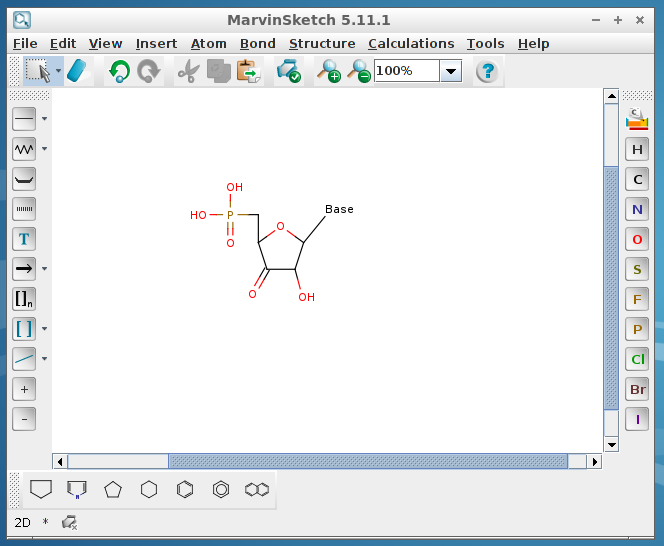
\includegraphics[width=0.5\textwidth]{ss-marvin-sketch.png}
		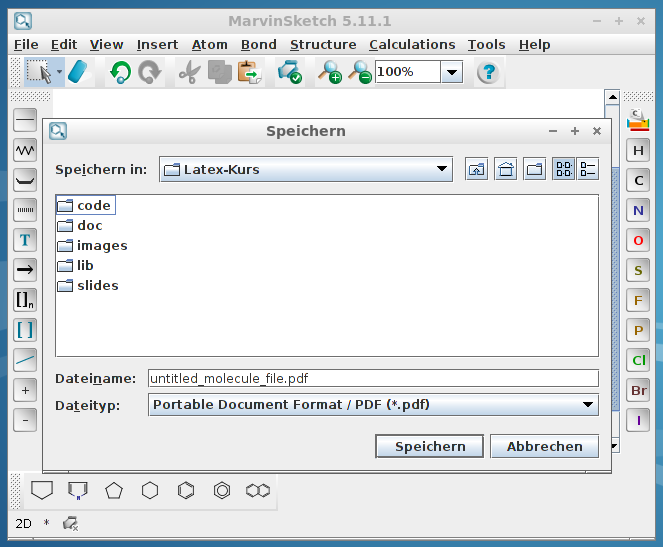
\includegraphics[width=0.5\textwidth]{ss-marvin-sketch-2.png}
	\end{center}
	ChemAxons Marvin Suite\footnote{\url{http://www.chemaxon.com}} (including Sketch) is freely available for academic
	use (Java).
\end{frame}


\section{Troubleshooting and remarkable problems}

\subsection{Too many packages added}
\begin{frame}
	While including many different packages, an error may occure:
		\code{! No room for a new \textbackslash{}dimen .
			\textbackslash{}ch@ck ...\textbackslash{}else
			\textbackslash{}errmessage \{No room for
		a new \#3\}}
	this can be prevented if the $\epsilon$-package can be added:
	\code{\textbackslash{}usepackage\{etex\}}
\end{frame}

\end{document}
